% SITUACIÓN DE APRENDIZAJE
\chapter{Unidad de trabajo: Seguridad en dispositivos domóticos de bajo coste}

\section*{Justificación y contexto}

En el contexto del módulo de \textit{Instalaciones Domóticas}, esta unidad de trabajo surge de la necesidad de reflexionar sobre la seguridad de los dispositivos conectados que se están integrando cada vez más en los hogares. Si bien su bajo coste y facilidad de uso son ventajas evidentes, su uso sin conocimientos mínimos de configuración segura puede suponer un riesgo importante. A través de esta unidad se pretendía generar conciencia crítica en el alumnado, vinculando el contenido técnico del módulo con aspectos de actualidad como la ciberseguridad, la privacidad y el diseño responsable de sistemas.

\section*{Contribución a las competencias profesionales}

La unidad contribuye al desarrollo de los resultados de aprendizaje recogidos en el currículo oficial del módulo (según el RD 177/2008 y la Orden de 2009 de la Comunitat Valenciana), especialmente aquellos vinculados a la instalación, configuración y mantenimiento de sistemas domóticos. Además, permite trabajar competencias clave como la digital, el pensamiento crítico y la resolución de problemas, incorporando un enfoque activo, práctico y participativo.

\section*{Resultados de aprendizaje trabajados}

\begin{itemize}
  \item Identificar los riesgos de seguridad asociados a dispositivos domóticos de bajo coste.
  \item Configurar entornos de red locales simulados sin conexión a Internet.
  \item Acceder, analizar y modificar parámetros básicos de dispositivos conectados.
  \item Valorar buenas prácticas de seguridad en instalaciones domóticas.
\end{itemize}

\section*{Desarrollo metodológico y actividades}

La unidad comenzó con una sesión teórica de contextualización, apoyada en la presentación digital \textit{Domótica de bajo coste: ¿comodidad inteligente o riesgo silencioso?}, que incluía preguntas orales al grupo y varios vídeos breves de YouTube sobre ataques reales y vulnerabilidades en hogares conectados.

Como dinámica inicial, se planteó una actividad de \textbf{icebreaker} en la que los alumnos, a través de un código QR proyectado, accedieron a una nube de palabras donde debían escribir nombres de dispositivos domóticos de bajo coste que conocían o tenían en casa. Curiosamente, antes de sacar el móvil para participar, varios estudiantes miraron a mi tutor como pidiendo permiso, lo que contrasta con su uso habitual del teléfono móvil con fines personales durante las clases, donde tienden a ocultarlo discretamente. A continuación, se muestra el resultado de la nube de palabras generada por el alumnado:
\begin{figure}[H]
  \centering
  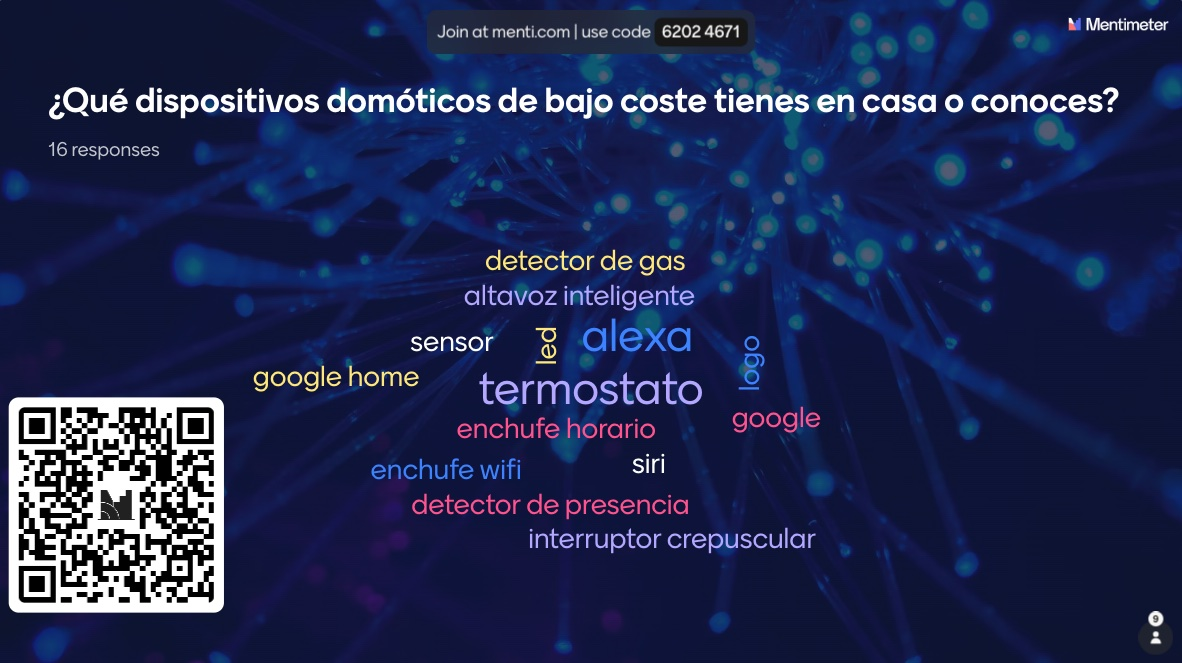
\includegraphics[width=0.8\textwidth]{resources/nube.jpg}
  \caption{Nube de palabras generada por el alumnado}
  \label{fig:nube_palabras}
\end{figure}

La actividad práctica se diseñó como una experiencia inmersiva en la que el alumnado debía simular un ataque ético. Para ello, se creó una red WiFi local con un router sin acceso a Internet, bajo el SSID “RedDomotica”, con una contraseña débil predefinida. El alumnado, trabajando en equipos, debía intentar acceder a la red, localizar un dispositivo Shelly Plug conectado, descubrir su IP y modificar su configuración sin utilizar la app oficial. 

Durante esta práctica se dieron varias situaciones destacables. Uno de los alumnos logró acceder a la configuración del router y cambió el nombre del SSID, lo que provocó que el dispositivo domótico dejara de estar accesible. Al final de la sesión, este mismo alumno se acercó a mí, algo preocupado, para confesar que había sido él quien lo había hecho, preguntando si había causado demasiados problemas. Le respondí que, si bien no era parte del plan, había sido una oportunidad valiosa para aprender de forma real y directa sobre los efectos de una mala configuración o un acceso no autorizado. 

También surgieron dificultades técnicas no previstas: no era posible acceder simultáneamente a la configuración del router desde varios dispositivos, lo cual ralentizó la actividad. Además, al intentar aplicar un ataque de fuerza bruta prolongado, el router se bloqueó temporalmente, lo que reforzó la comprensión del alumnado sobre los riesgos reales de este tipo de ataques.

\section*{Materiales y recursos utilizados}

\begin{itemize}
  \item Presentación digital en formato PDF.
  \item Pizarra digital interactiva SYNETECH Advance Aquarius (modelo A7532).
  \item Router configurado sin conexión a Internet (SSID: RedDomotica).
  \item Enchufe inteligente Shelly Plug.
  \item Dispositivos móviles y ordenadores personales del alumnado.
\end{itemize}

\section*{Evaluación}

La evaluación de esta unidad de trabajo se integró como parte del examen del módulo. Se incluyeron tres preguntas tipo test (valoradas en 0,2 puntos cada una) que abordaban conceptos clave tratados en las sesiones:

\begin{enumerate}
  \item ¿Qué tipo de ataque compromete la disponibilidad de un sistema domótico mediante la sobrecarga de la red o del servidor? (Correcta: c) Denegación de Servicio (DoS)).
  \item ¿Cuál de las siguientes opciones se puede considerar mala praxis a la hora de configurar una instalación de dispositivos de bajo coste? (Correcta: d) Todas las opciones se pueden considerar mala praxis).
  \item ¿Qué significa que un sistema domótico tenga baja escalabilidad? (Correcta: b) Que tiene dificultades para integrar nuevos dispositivos o tecnologías en el futuro).
\end{enumerate}

\section*{Adaptaciones y atención a la diversidad}

No fue necesario aplicar adaptaciones curriculares durante esta unidad. Al tratarse de Formación Profesional, las adaptaciones de acceso sólo se contemplan en casos muy concretos, y en este grupo no se dio ninguna situación que las requiriera. Tampoco se aplicaron criterios del Diseño Universal para el Aprendizaje (DUA), más allá de ofrecer información por vía visual y oral, lo cual forma parte del enfoque habitual en este tipo de módulos.

\section*{Valoración final}

La experiencia resultó altamente enriquecedora, tanto por el grado de implicación del alumnado como por la oportunidad de conectar los contenidos curriculares con la realidad tecnológica del presente. La unidad permitió trabajar competencias clave, fomentar el pensamiento crítico y abrir un espacio para la reflexión ética en el ámbito profesional. Aunque surgieron imprevistos técnicos, estos no solo no perjudicaron la sesión, sino que sirvieron como catalizador para un aprendizaje más profundo y significativo.



% \chapter{Propuesta didáctica: Domótica de Bajo Coste}
% \section{Justificación y Contexto}
% El uso de dispositivos domóticos de bajo coste está en auge, pero la seguridad sigue siendo un aspecto desatendido. Esta SA busca concienciar a los alumnos sobre las vulnerabilidades de estos sistemas.

% \section{Objetivos}
% \begin{itemize}
%     \item Comprender los riesgos de seguridad en la domótica de bajo coste.
%     \item Identificar vulnerabilidades en dispositivos IoT.
%     \item Aplicar buenas prácticas de configuración segura.
% \end{itemize}

% \section{Contenidos}
% \begin{itemize}
%     \item Seguridad en redes WiFi y dispositivos inteligentes.
%     \item Métodos de ataque: fuerza bruta, sniffing, spoofing.
%     \item Configuración de dispositivos domóticos seguros.
% \end{itemize}

% \section{Desarrollo de la sesión}
% \textbf{1. Teoría (1h)}  
% Explicación sobre vulnerabilidades en domótica y medidas de protección.

% \textbf{2. Práctica (1h 45min)}  
% \begin{itemize}
%     \item Configuración de un enchufe inteligente Shelly Plug.
%     \item Simulación de ataques a una red WiFi insegura.
%     \item Análisis de permisos de aplicaciones domóticas.
% \end{itemize}

% \section{Evaluación}
% \begin{itemize}
%     \item Participación en la sesión (30\%).
%     \item Realización de la práctica (40\%).
%     \item Examen tipo test (30\%).
% \end{itemize}